
\section{Results and Analysis}
\subsection{Qualitative results}
\Cref{fig:best-qualitative-a,fig:best-qualitative-b} shows the best selected result for each image according to own-GT macro IoU. The full appendix includes the complete output gallery with all 478 post-processed result cases. In the main report, these selected examples show how the feature-space combinations behave across different images.

\begin{figure}[H]
\centering
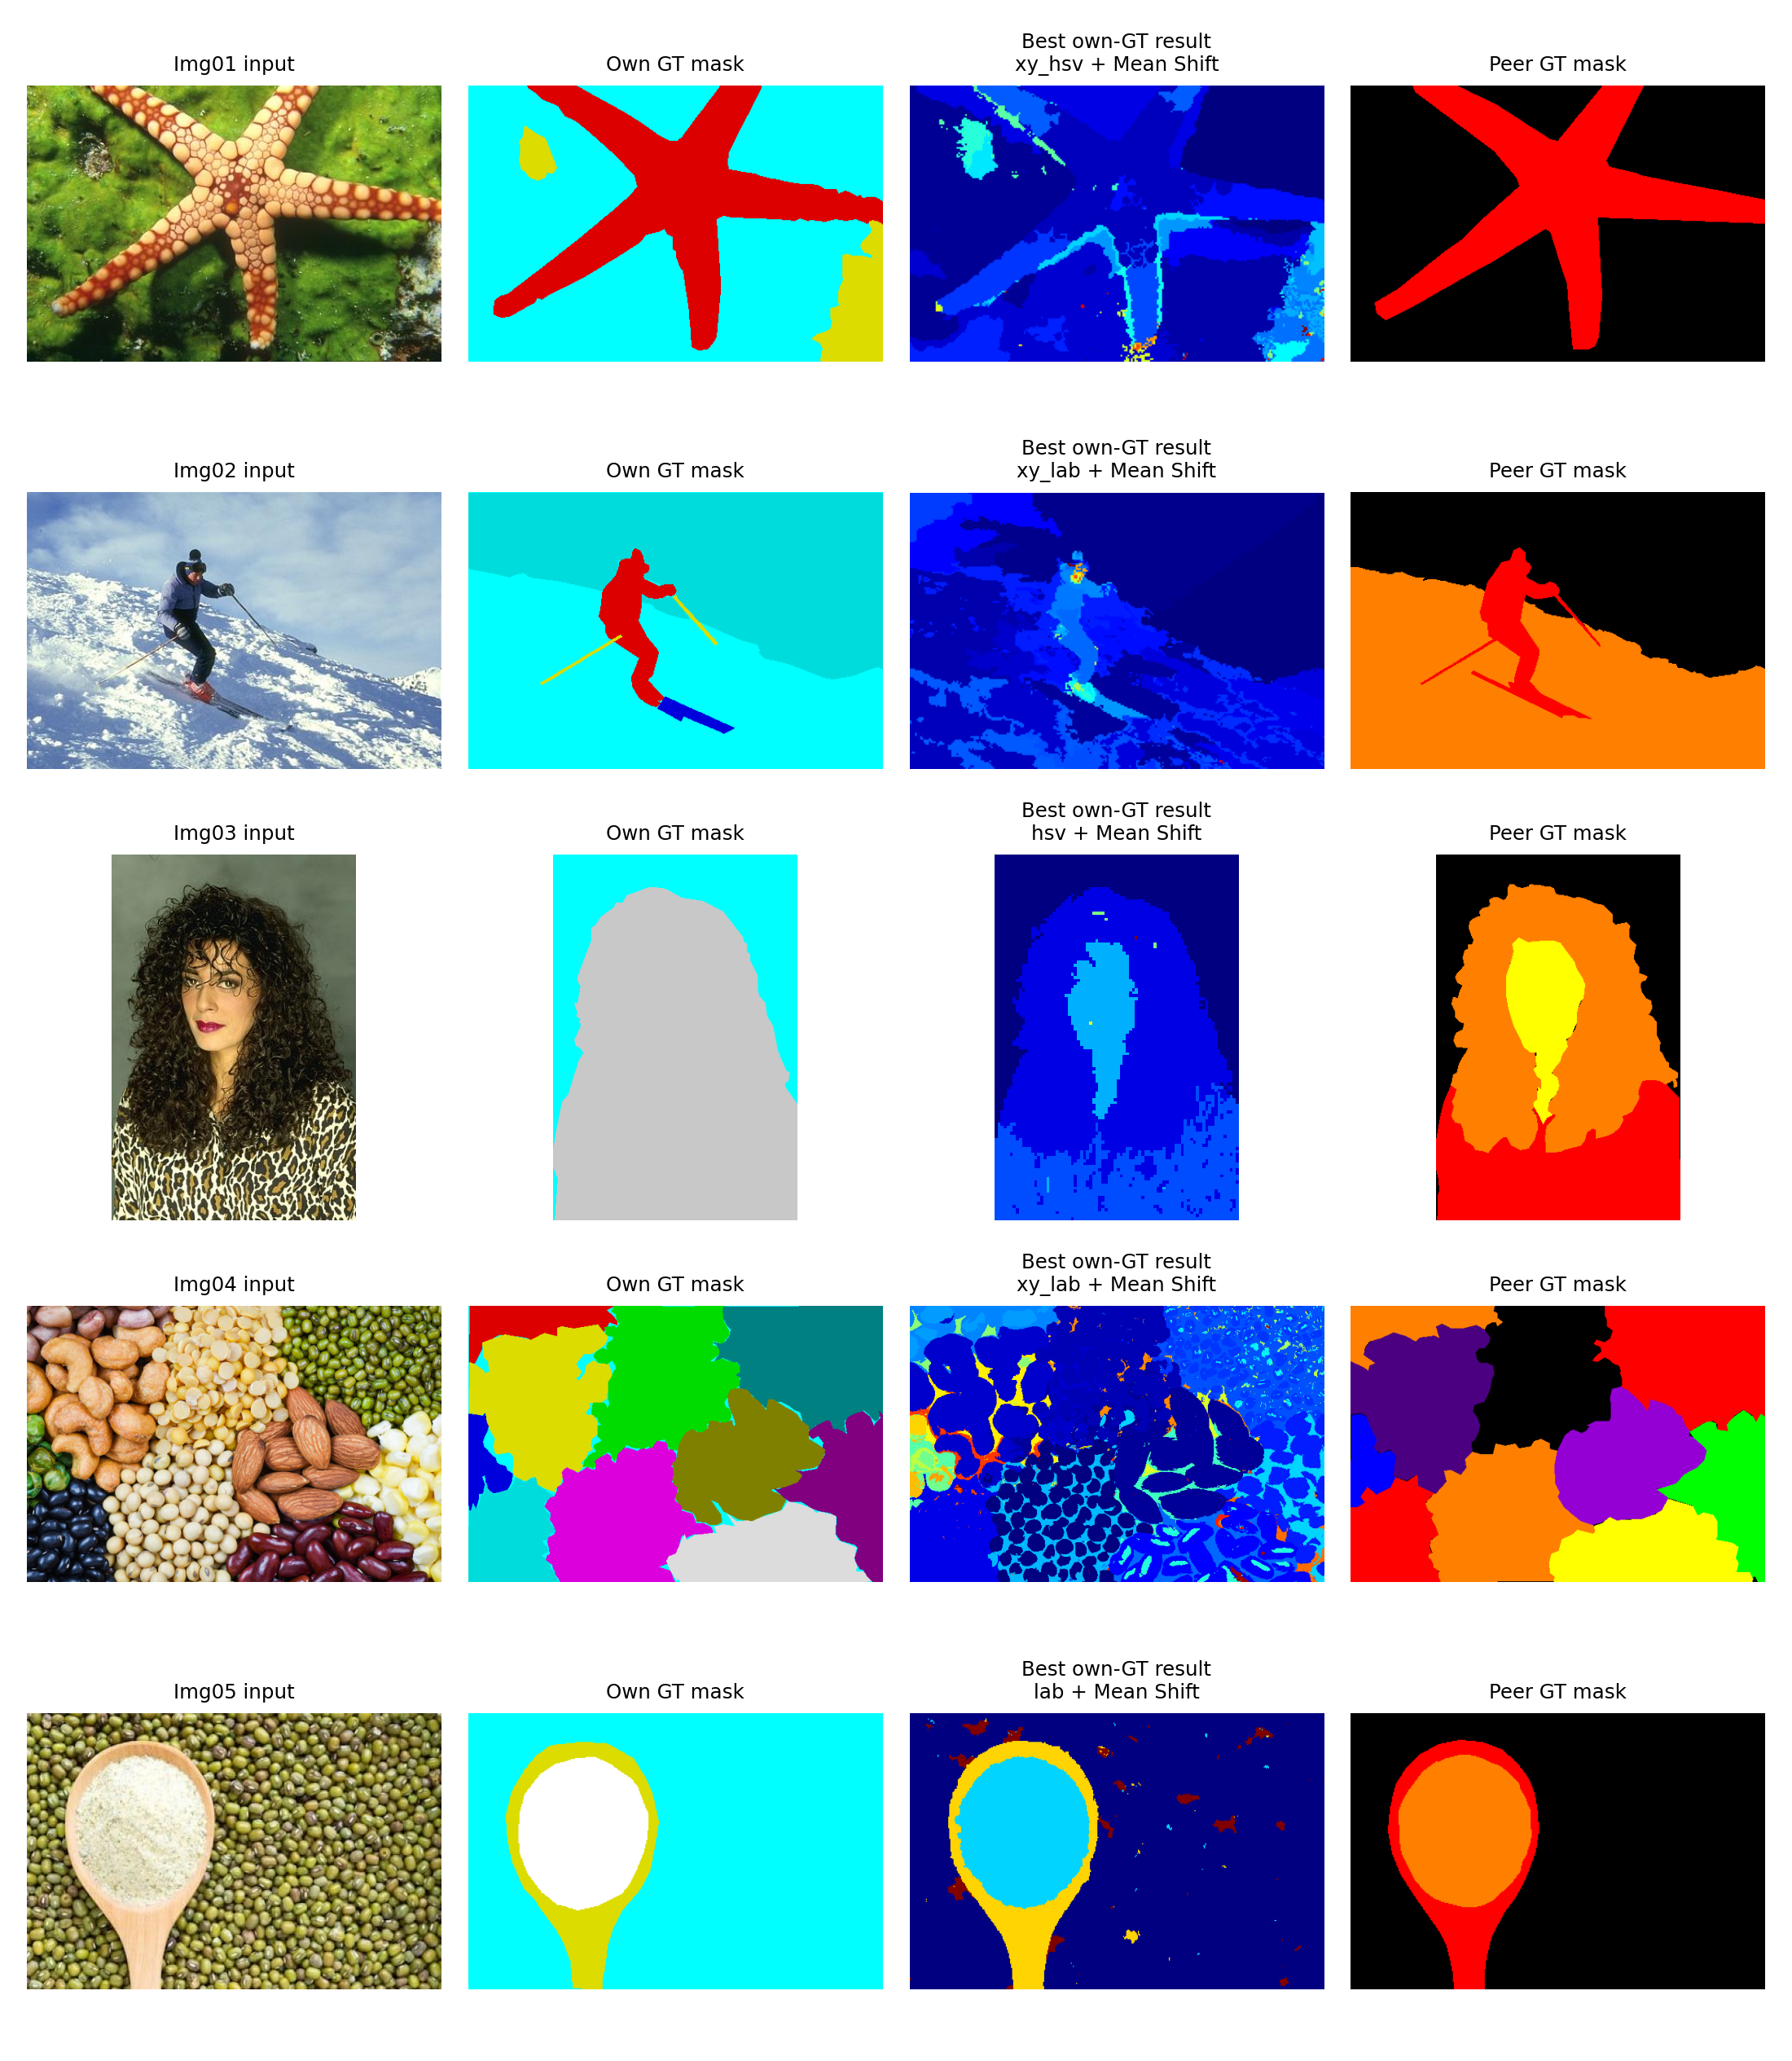
\includegraphics[width=0.95\textwidth,height=0.43\textheight,keepaspectratio]{figures/grids/best_qualitative_results_part1.png}
\caption{Best qualitative segmentation examples for Images 01--05, selected per image using own-GT macro IoU. Each row shows the input, own GT mask, selected machine output, and peer GT mask.}
\label{fig:best-qualitative-a}
\end{figure}
\begin{figure}[H]
\centering
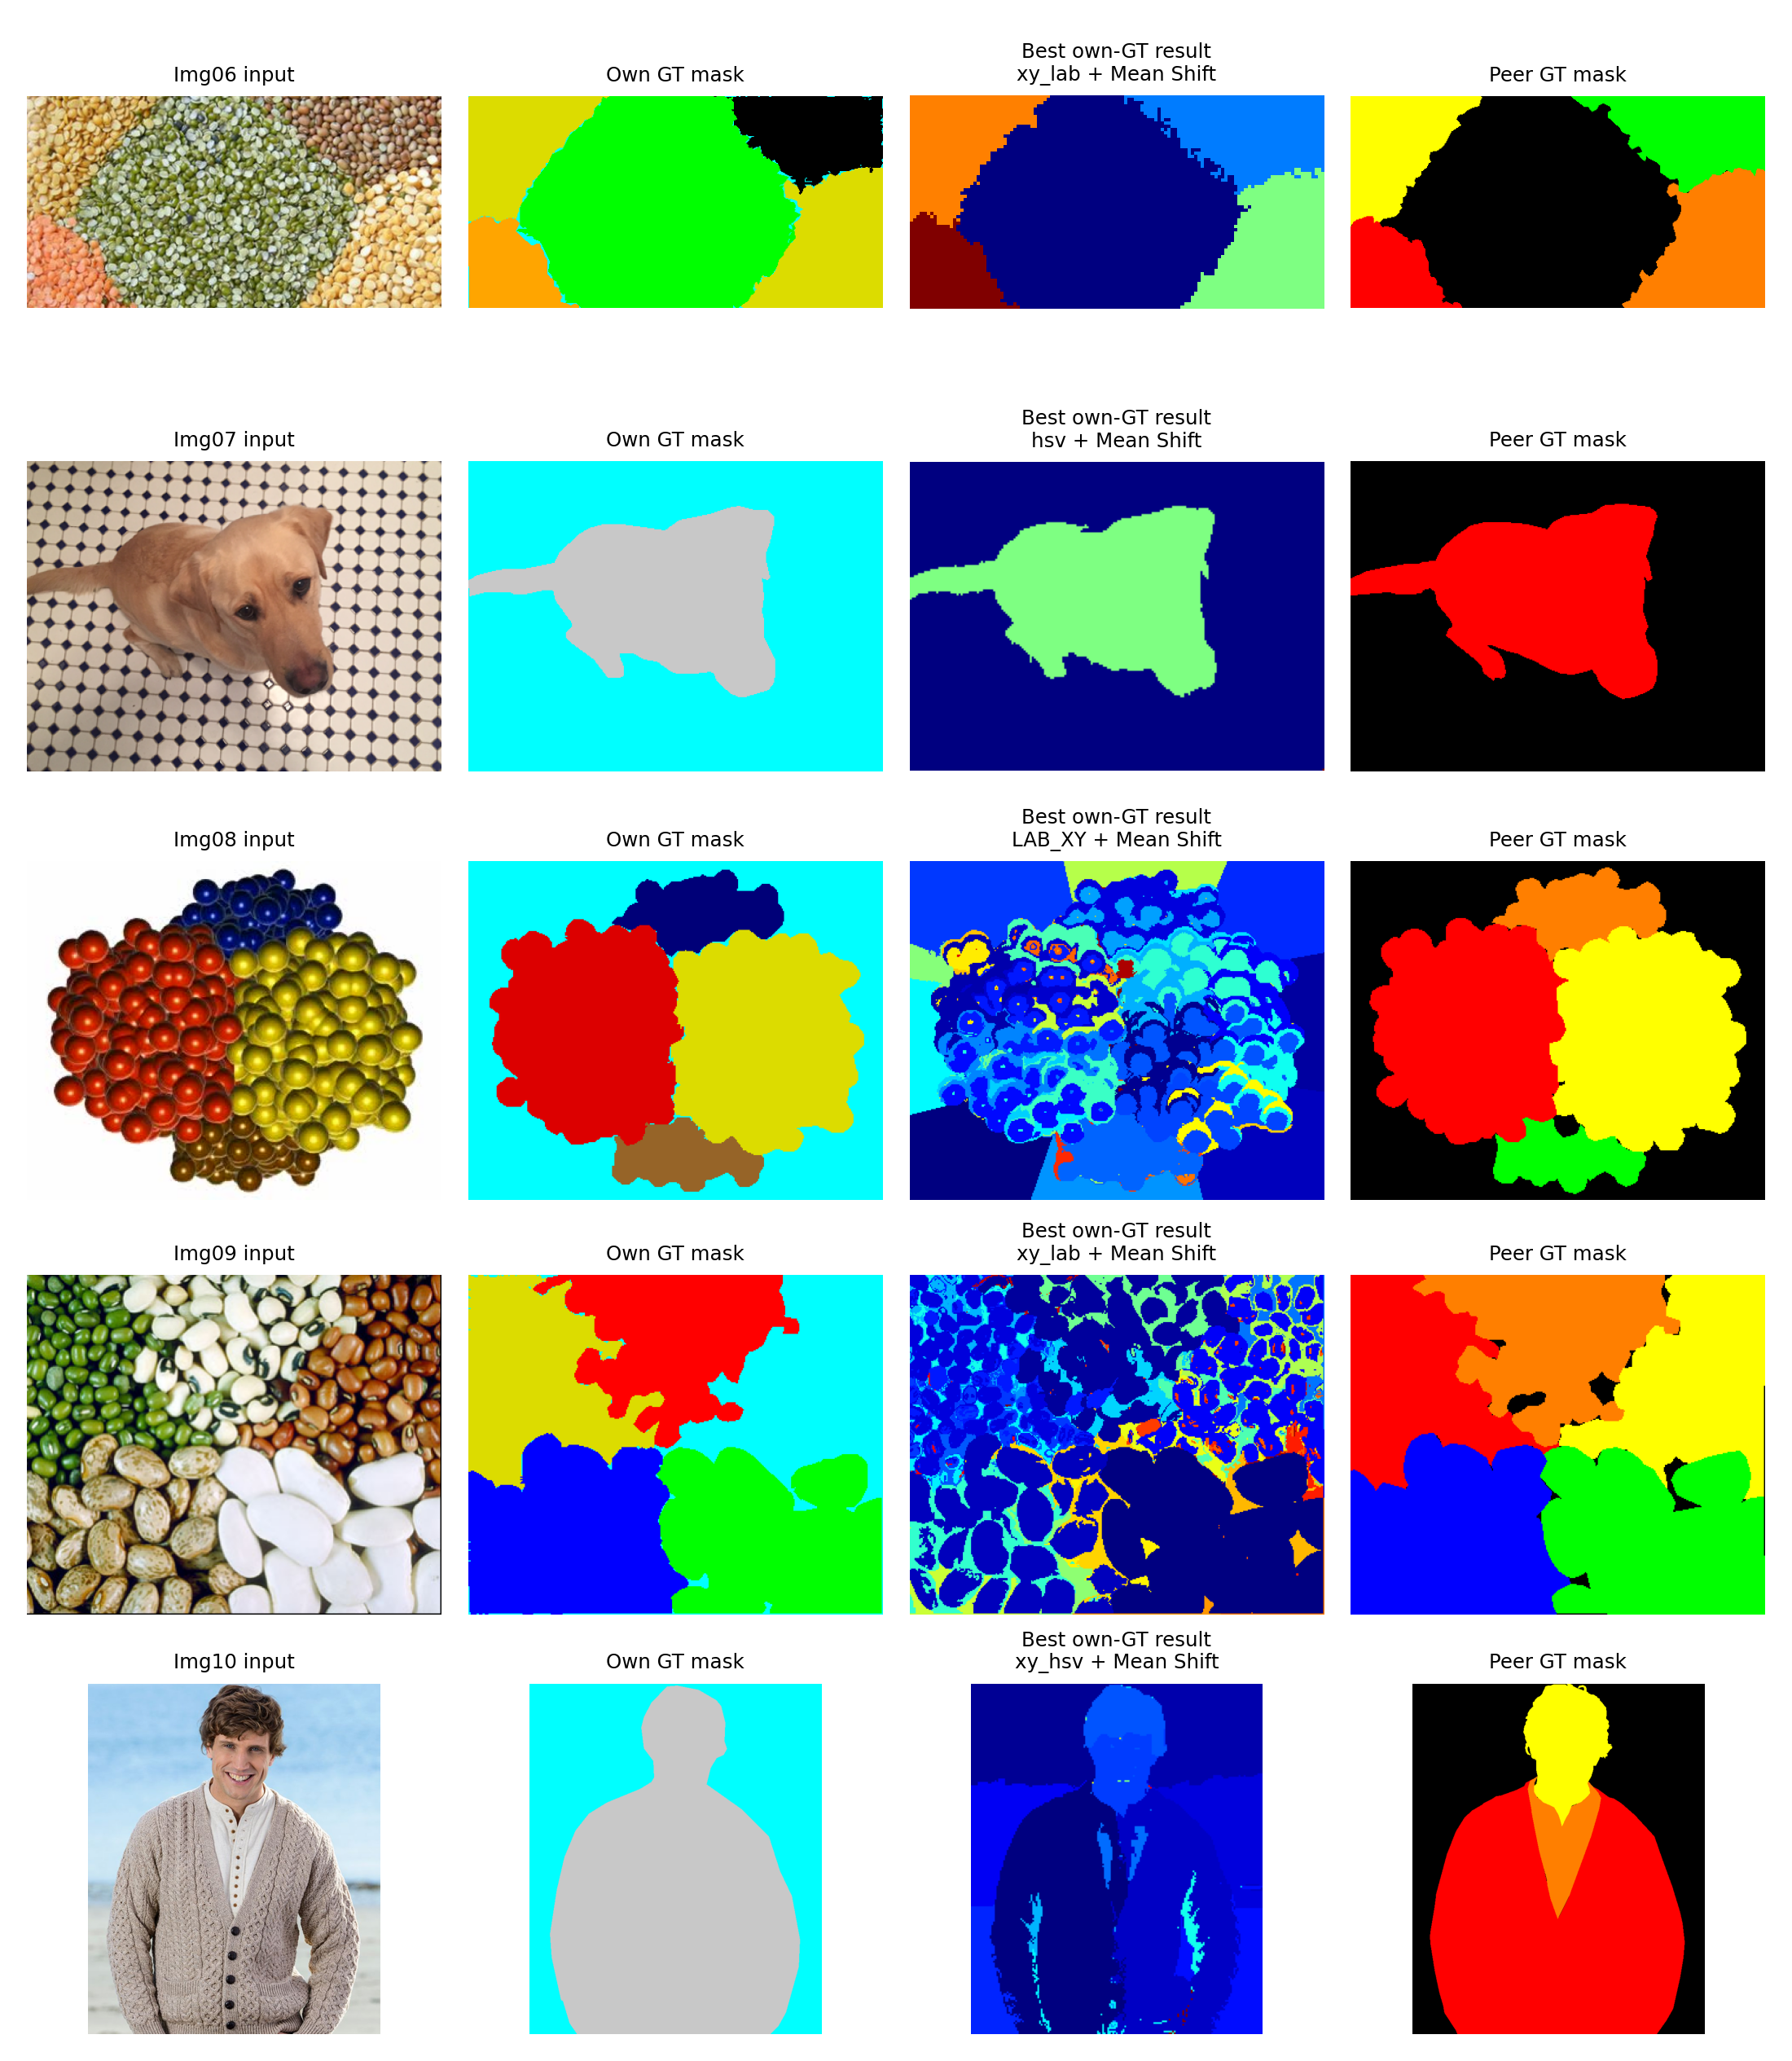
\includegraphics[width=0.95\textwidth,height=0.43\textheight,keepaspectratio]{figures/grids/best_qualitative_results_part2.png}
\caption{Best qualitative segmentation examples for Images 06--10, selected per image using own-GT macro IoU.}
\label{fig:best-qualitative-b}
\end{figure}

\subsection{Quantitative summary}
Across all 478 post-processed outputs, the overall macro Precision is 0.588, macro Recall is 0.601, macro IoU is 0.498, and macro Boundary F1-score is 0.257. These averages include deliberately weak feature spaces, under-segmented outputs, over-segmented outputs, and multiple Mean Shift bandwidths, so they represent the full experimental sweep rather than only the best cases.

\begin{figure}[H]
\centering
\begin{subfigure}{0.48\textwidth}
\centering
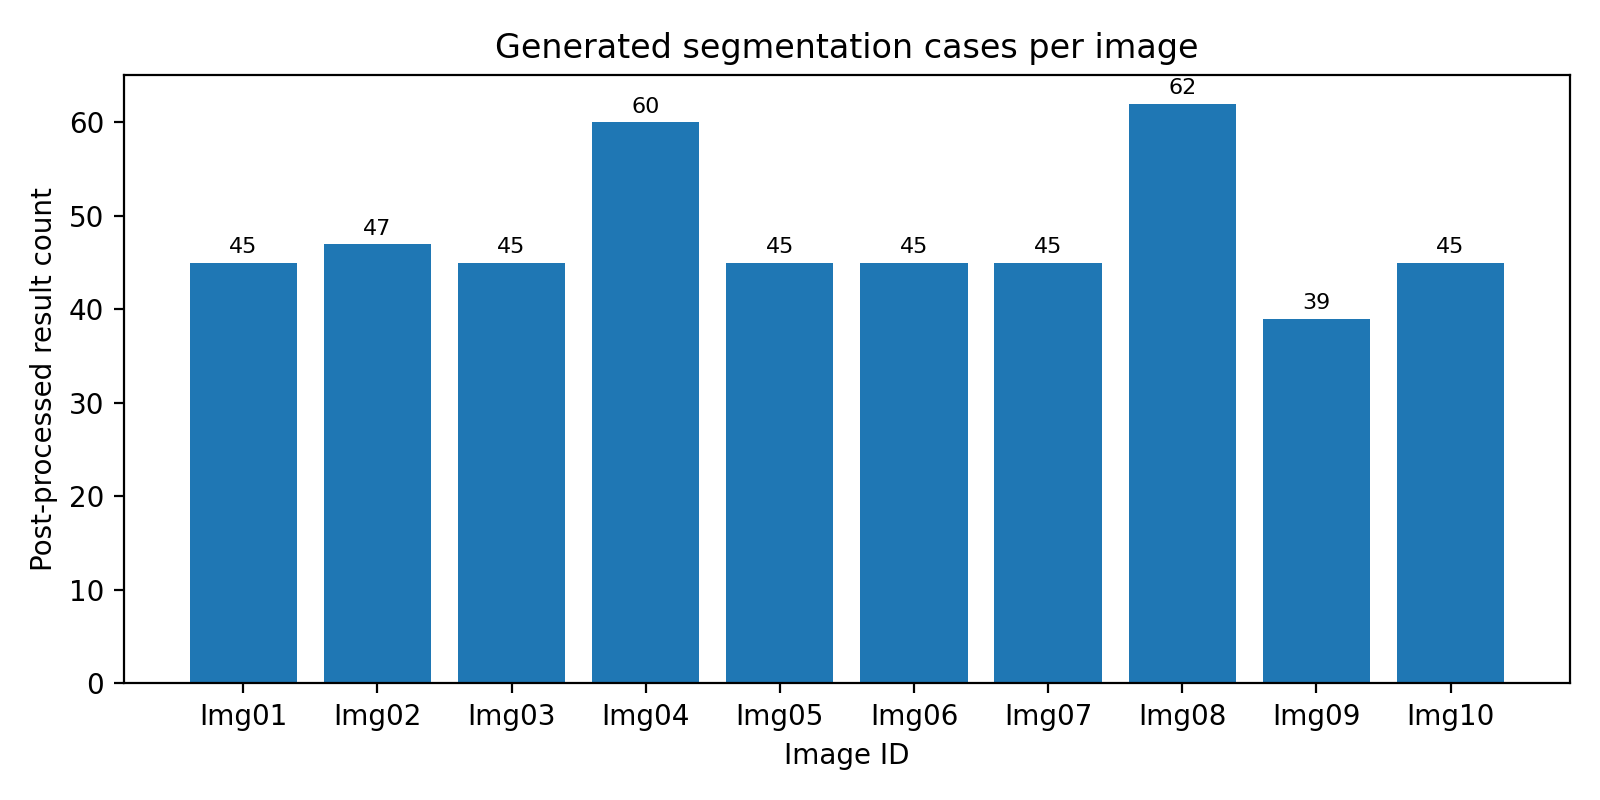
\includegraphics[width=\textwidth]{figures/charts/output_count_by_image.png}
\caption{Number of generated result cases per image.}
\end{subfigure}\hfill
\begin{subfigure}{0.48\textwidth}
\centering
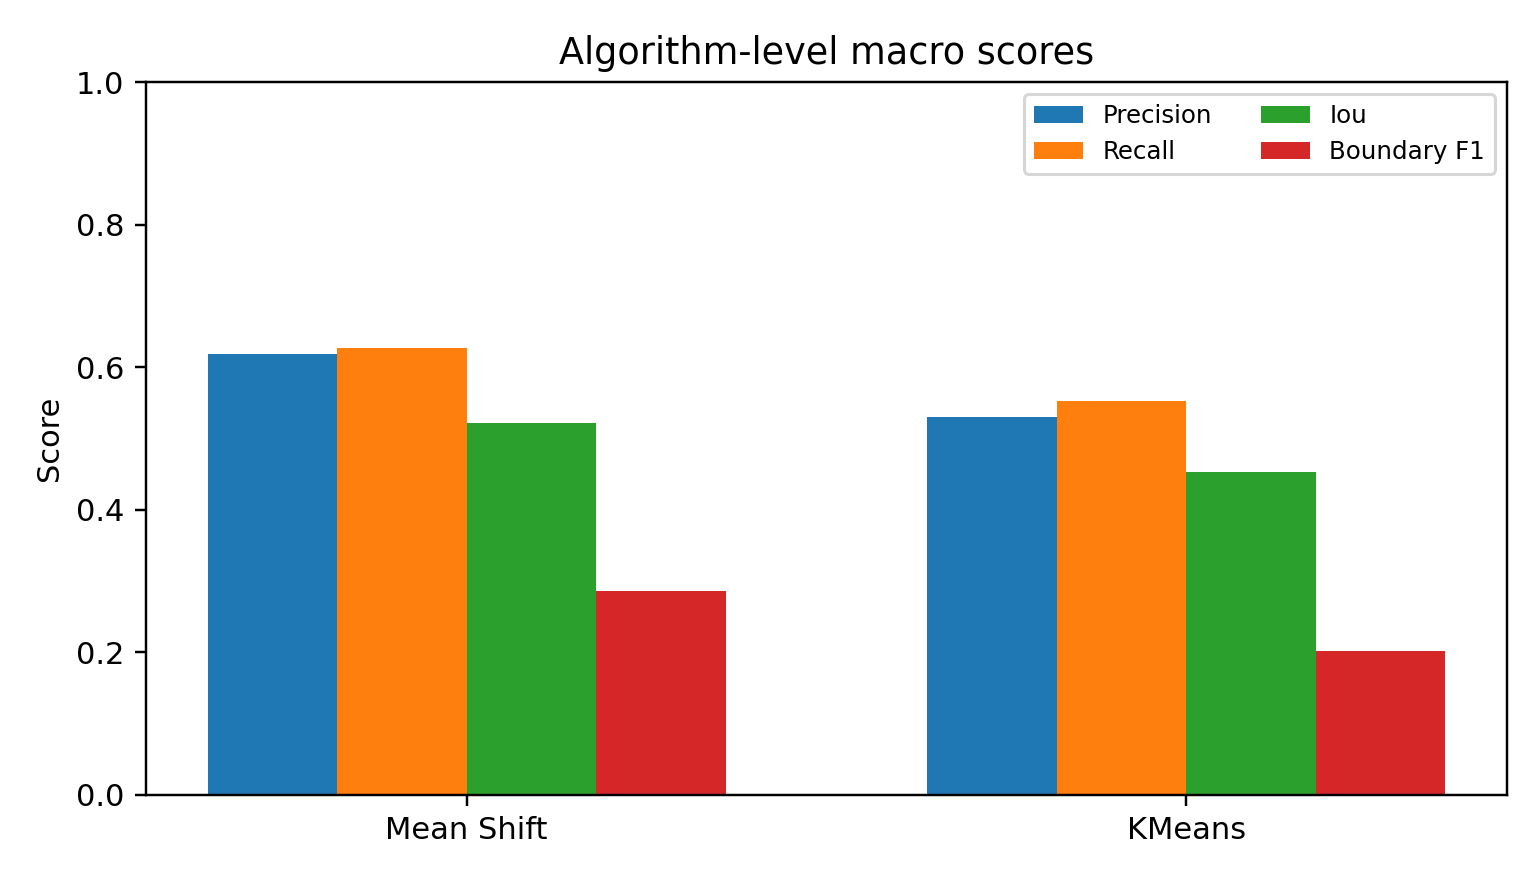
\includegraphics[width=\textwidth]{figures/charts/algorithm_summary_metrics.png}
\caption{Macro scores grouped by algorithm.}
\end{subfigure}
\caption{Quantitative overview of the complete experiment.}
\label{fig:quant-overview}
\end{figure}

\begin{table}[H]
\centering
\caption{Algorithm-level quantitative results over the generated outputs.}
\resizebox{\textwidth}{!}{%
\begin{tabular}{@{}lrrrrrr@{}}
\toprule
Algorithm & Cases & Images & Prec. & Recall & IoU & BF \\
\midrule
Mean Shift & 314 & 10 & 0.619 & 0.626 & 0.521 & 0.285 \\
KMeans & 164 & 10 & 0.530 & 0.553 & 0.454 & 0.202 \\
\bottomrule
\end{tabular}
}
\label{tab:algorithm-results}
\end{table}

\subsection{Best feature-space groups}
The strongest feature-space groups combine spatial coordinates with Lab or HSV color, and in some cases texture. This supports the design idea: spatial features improve compactness, while perceptual color spaces make the clusters more meaningful than raw RGB alone.

\begin{figure}[H]
\centering
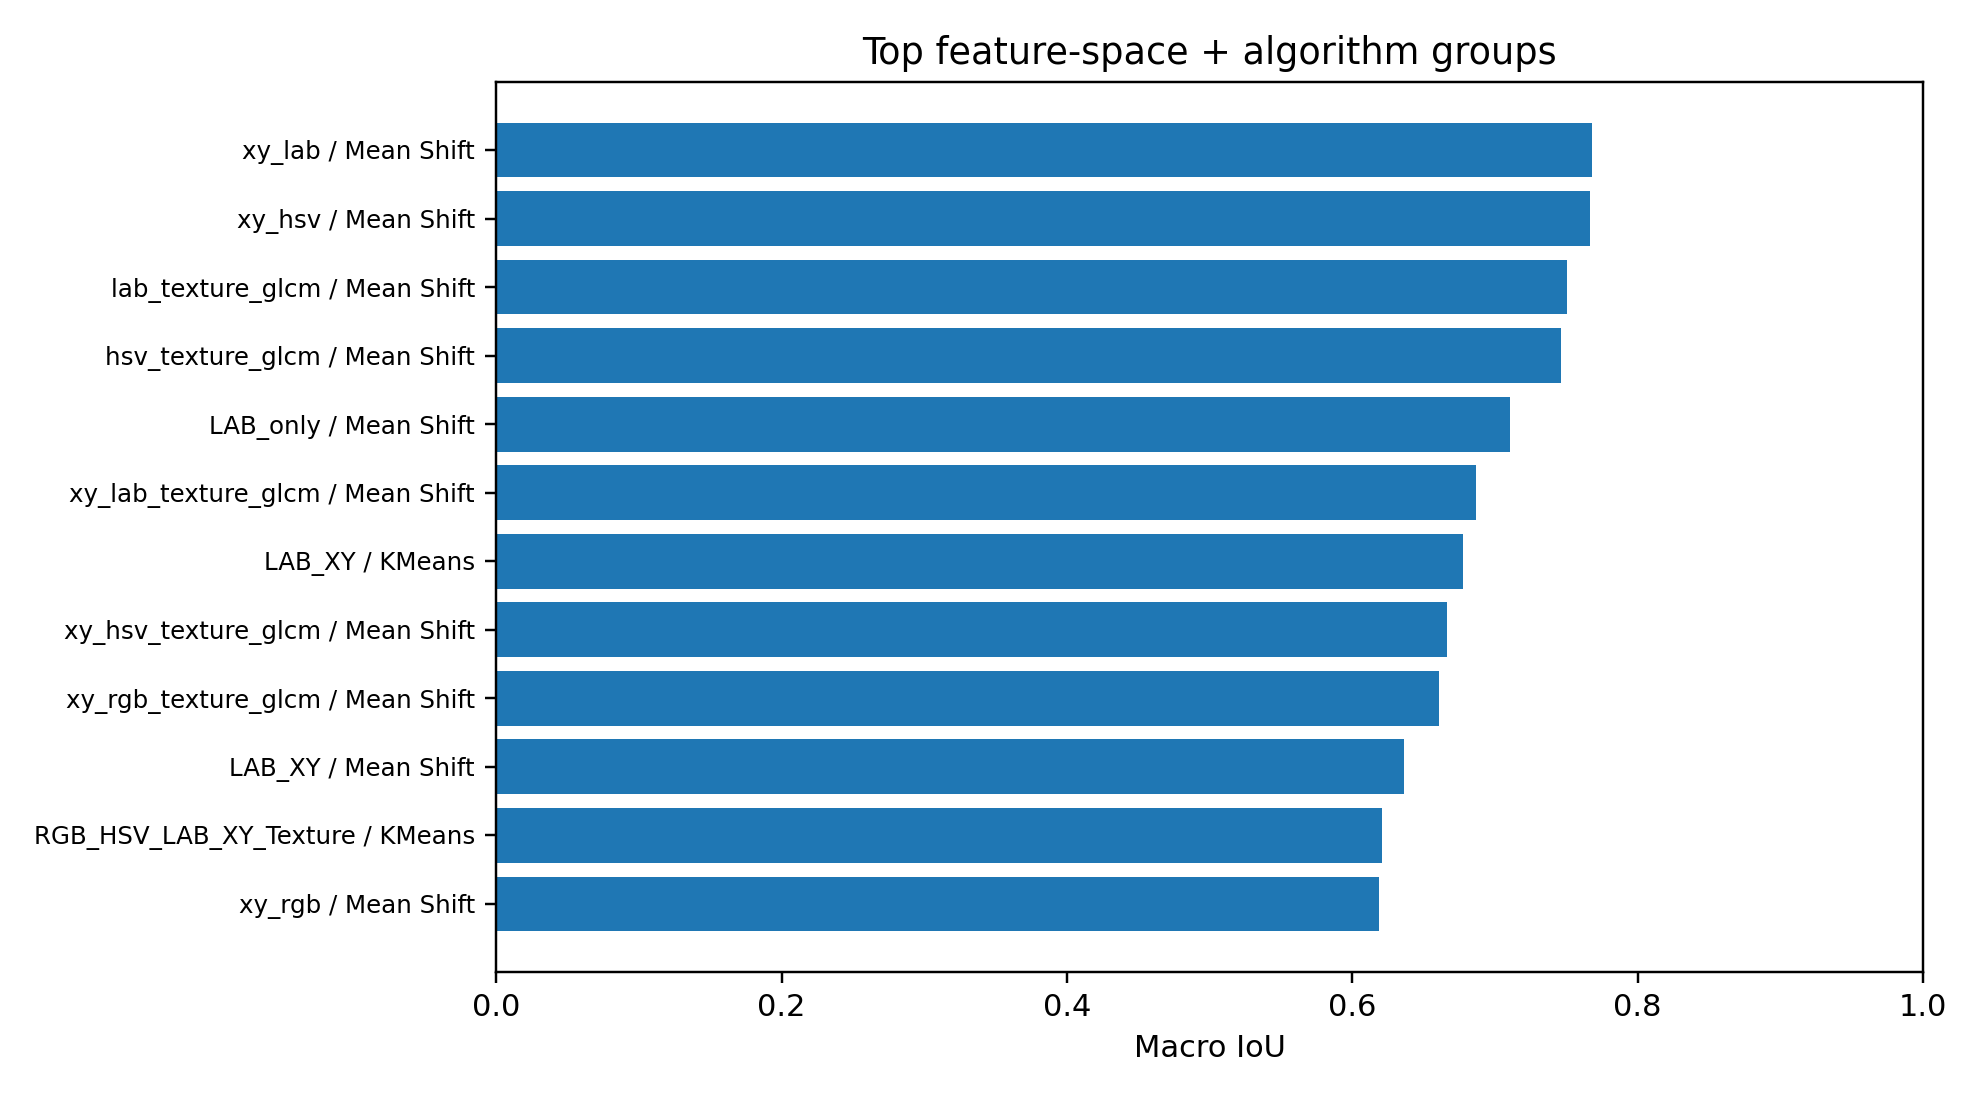
\includegraphics[width=0.9\textwidth]{figures/charts/top_feature_algorithm_macro_iou.png}
\caption{Top feature-space and algorithm groups ranked by macro IoU.}
\label{fig:top-feature-algorithm}
\end{figure}

\begin{table}[H]
\centering
\caption{Top feature-space and algorithm groups by macro IoU.}
\resizebox{\textwidth}{!}{%
\begin{tabular}{@{}lrrrrrrr@{}}
\toprule
Feature set & Alg. & Cases & Images & Prec. & Recall & IoU & BF \\
\midrule
xy\_lab & Mean Shift & 18 & 9 & 0.825 & 0.821 & 0.768 & 0.514 \\
xy\_hsv & Mean Shift & 18 & 9 & 0.833 & 0.825 & 0.767 & 0.501 \\
lab\_texture\_glcm & Mean Shift & 6 & 3 & 0.848 & 0.796 & 0.750 & 0.446 \\
hsv\_texture\_glcm & Mean Shift & 6 & 3 & 0.822 & 0.816 & 0.746 & 0.434 \\
LAB\_only & Mean Shift & 6 & 1 & 0.747 & 0.789 & 0.711 & 0.552 \\
xy\_lab\_texture\_glcm & Mean Shift & 6 & 3 & 0.800 & 0.741 & 0.687 & 0.430 \\
LAB\_XY & KMeans & 1 & 1 & 0.699 & 0.727 & 0.678 & 0.482 \\
xy\_hsv\_texture\_glcm & Mean Shift & 6 & 3 & 0.820 & 0.731 & 0.666 & 0.429 \\
\bottomrule
\end{tabular}
}
\label{tab:top-feature-algorithm}
\end{table}

\subsection{Representative normalized confusion matrix}
The normalized confusion matrix in \Cref{fig:representative-cm} shows a representative best-scoring result. Values on the diagonal correspond to correctly matched GT classes, while off-diagonal entries show class confusion after label matching. The complete long-form normalized confusion matrices are included in \texttt{numerical\_results/own\_gt/confusion\_matrices\_long.csv}.

\begin{figure}[H]
\centering
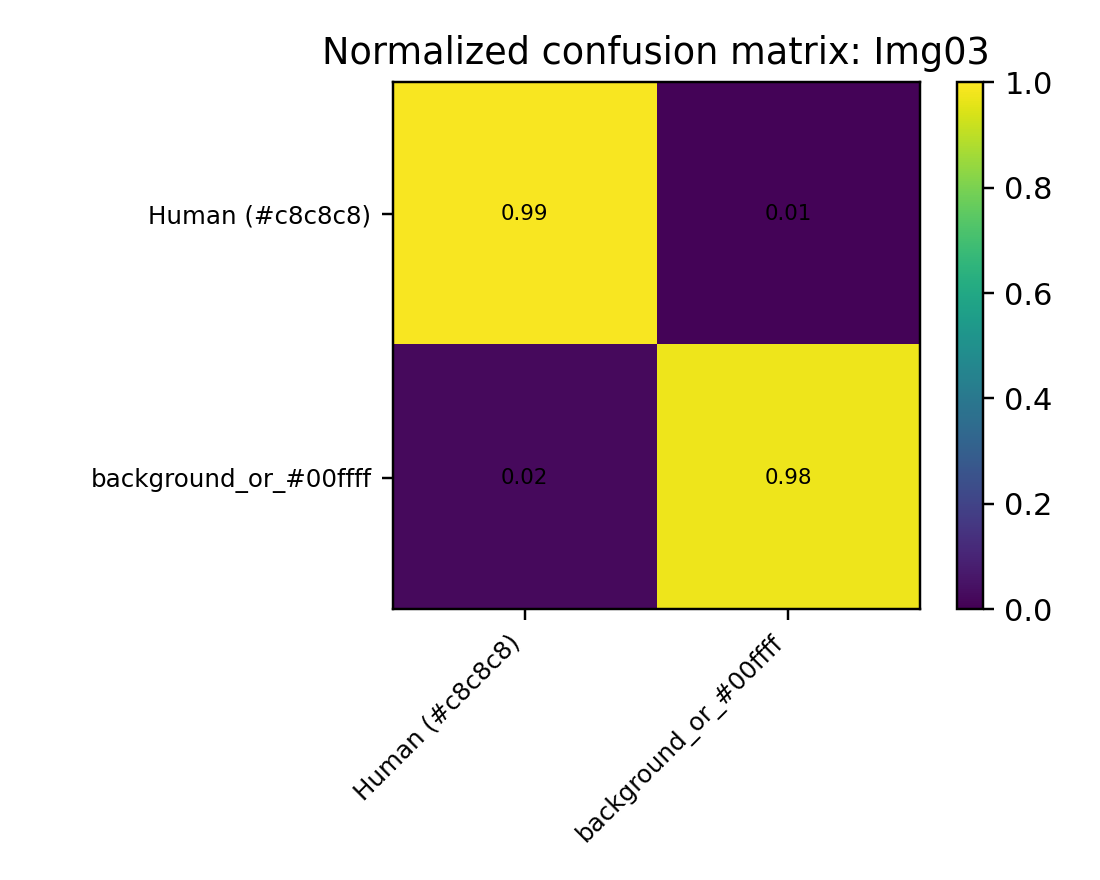
\includegraphics[width=0.58\textwidth]{figures/charts/representative_confusion_matrix.png}
\caption{Representative row-normalized confusion matrix after many-to-one label matching.}
\label{fig:representative-cm}
\end{figure}

\subsection{Discussion}
Several trends are visible in the output tables and figures. First, XY combined with Lab or HSV is consistently strong, because it balances color discrimination with spatial coherence. Second, texture-only features can be useful when surface pattern dominates, but they may be unstable when the image contains smooth regions or when Mean Shift produces too many small modes. Third, K-means is fast and stable but depends on a chosen $K$, while Mean Shift can adapt cluster count but needs careful bandwidth, sampling, resizing, or PCA. Finally, post-processing improves visual smoothness by removing isolated components, which is important because unsupervised clustering often produces small noisy islands.
